% Primeira revisão, Fase 2: Introdução e visão geral (capítulos 1--4).
% Figuras originais provenientes de mb-uso/figuras no acervo da monografia.
% Material de trabalho: sem os exemplos (capítulos 5 e 6).

\begin{frame}[plain]
\vspace{.85cm}
{\Large\color{navy}Um framework analítico extensível para benchmarking de algoritmos evolutivos multiobjetivo\par}
\vspace{.65cm}
{\large Fernando Ferreira da Silva\par}
\vspace{.2cm}Dissertação de Mestrado --- PPG-CCMC\par
\vspace{.42cm}Instituto de Ciências Matemáticas e de Computação --- Universidade de São Paulo\par
Orientador: Prof. Dr. Francisco José Monaco
\end{frame}

\begin{frame}[plain]
\vspace{1.8cm}{\LARGE\color{navy}Introdução\par}\vspace{.3cm}\textcolor{navy!40}{\rule{.76\linewidth}{.65pt}}
\end{frame}

\begin{frame}{Problemas multiobjetivo e dominância de Pareto}
\begin{columns}[T,onlytextwidth]
\begin{column}{.53\textwidth}
Uma solução de um problema multiobjetivo é avaliada simultaneamente por várias funções que podem ser conflitantes.
\[
\min_{x\in\Omega}\; f(x)=\bigl(f_1(x),\ldots,f_M(x)\bigr)
\]
Para minimização, $x$ domina $y$ quando não é pior em nenhum objetivo e é melhor em pelo menos um:
\[
x\prec y\iff\bigl(\forall i:f_i(x)\le f_i(y)\bigr)\land
\bigl(\exists j:f_j(x)<f_j(y)\bigr).
\]
\end{column}
\begin{column}{.45\textwidth}
\centering
\begin{tikzpicture}[x=0.65cm,y=0.65cm,>=stealth]
\draw[->,thick] (0,0)--(6.1,0) node[below]{$f_1$};
\draw[->,thick] (0,0)--(0,5.2) node[left]{$f_2$};
\draw[navy,very thick] plot[smooth] coordinates{(0.8,4.55)(1.45,3.5)(2.5,2.55)(3.75,1.65)(5.2,0.95)};
\foreach \x/\y in {0.9/4.4,1.45/3.5,2.5/2.55,3.75/1.65,5.2/0.95}{\fill[navy] (\x,\y) circle (2.4pt);}
\foreach \x/\y in {2.2/4.25,3.0/3.5,4.6/2.9,4.9/4.2,5.4/2.0}{\fill[black!35] (\x,\y) circle (2.4pt);}
\node[align=left,text=navy,font=\scriptsize] at (3.1,4.8){não dominadas};
\draw[->,navy] (2.5,4.6)--(1.45,3.65);
\node[align=left,font=\scriptsize,text=black!65] at (4.9,3.65){dominadas};
\end{tikzpicture}
\vspace{.1cm}
{\scriptsize Esquema bidimensional ilustrativo; ambos os objetivos são minimizados.}
\end{column}
\end{columns}
\vspace{.15cm}
As soluções não dominadas formam alternativas de compromisso. Sua imagem no espaço de objetivos constitui a fronteira de Pareto.
\end{frame}

\begin{frame}{MOEAs e problemas com muitos objetivos}
Algoritmos evolutivos multiobjetivo (MOEAs) procuram aproximar a fronteira de Pareto mantendo uma população de soluções, em vez de retornar uma única alternativa.
\par\medskip
Com muitos objetivos (\textit{many-objective}), é comum que uma fração crescente da população seja mutuamente não dominada. Consequentemente, a dominância de Pareto perde poder discriminativo para orientar seleção e comparação.
\par\medskip
A avaliação passa a exigir indicadores complementares, protocolos estatísticos e recursos que funcionem também quando a fronteira não pode ser visualizada diretamente em duas ou três dimensões.
\end{frame}

\begin{frame}{Benchmarking de algoritmos evolutivos}
Uma avaliação experimental precisa estabelecer \textbf{qual problema é resolvido}, \textbf{em quais condições}, \textbf{como os resultados são medidos} e \textbf{como a variabilidade é tratada}.
\par\medskip
Um protocolo comparável envolve configurações explícitas, execuções repetidas, indicadores, referências comuns de normalização e análises estatísticas. A interpretação também depende de saber quais populações, gerações e espaços foram efetivamente examinados.
\par\medskip
Em problemas many-objective, o cálculo de alguns indicadores é computacionalmente caro; a escolha de procedimentos exatos ou aproximados também passa a integrar o protocolo.
\end{frame}

\begin{frame}{Motivação e posicionamento}
Bibliotecas como jMetal, PlatEMO e pymoo oferecem implementações importantes de problemas, algoritmos e recursos de avaliação.
\par\medskip
A motivação desta pesquisa é disponibilizar \textbf{uma camada de abstração para o trabalho experimental}, que reúna os componentes necessários a uma investigação em um modelo uniforme de configuração, execução e análise.
\par\medskip
O MoeaBench orquestra esses recursos e organiza reprodutibilidade, comparabilidade, persistência e interpretação, reduzindo a necessidade de programar repetidamente a infraestrutura de cada benchmark.
\end{frame}

\begin{frame}{Principais recursos previstos no MoeaBench}
\begin{tabularx}{\linewidth}{@{}>{\bfseries}p{.27\linewidth}X@{}}
Reprodutibilidade & Configurações, sementes por execução, sementes de componentes, ambiente e metadados são identificáveis e recuperáveis.\\[5pt]
Comparabilidade & Execuções repetidas, referências de normalização explícitas, indicadores e testes estatísticos.\\[5pt]
Análise & Visualizações espaciais, históricos de desempenho, comparações distribucionais e camadas de dominância.\\[5pt]
Extensibilidade & MOPs e MOEAs personalizados podem ser utilizados pela mesma interface experimental.\\[5pt]
Escalabilidade & Séries DTLZ e DPF; ausência de limites artificiais de objetivos ou variáveis; métodos especializados para cálculos custosos.\\[5pt]
Persistência & Arquivos de experimento que preservam resultados e informações necessárias à reanálise.\\
\end{tabularx}
\vspace{.13cm}{\scriptsize Fontes: monografia, capítulo 4; MoeaBench User Guide.}
\end{frame}

\begin{frame}{Objetivo da pesquisa}
Desenvolver o \textbf{MoeaBench}, um framework analítico extensível para benchmarking de algoritmos evolutivos multiobjetivo.
\par\bigskip
A proposta integra a definição do protocolo e a execução de MOEAs com a organização dos resultados, a avaliação quantitativa, a análise estatística, a visualização e o registro da proveniência científica.
\par\bigskip
A pesquisa também desenvolve recursos para avaliação em muitos objetivos e para a interpretação estruturada da qualidade das frentes aproximadas, apresentados em seções posteriores.
\end{frame}

\begin{frame}[plain]
\vspace{1.8cm}{\LARGE\color{navy}O MoeaBench\par}\vspace{.3cm}\textcolor{navy!40}{\rule{.76\linewidth}{.65pt}}
\end{frame}

\begin{frame}[fragile]{Experimento mínimo: configuração e execução}
\begin{columns}[T,onlytextwidth]
\begin{column}{.45\textwidth}
O experimento reúne o problema, o algoritmo e os resultados da execução.
\begin{lstlisting}[style=python,basicstyle=\ttfamily\fontsize{8}{10}\selectfont]
import moeabench as mb

exp = mb.experiment()
exp.mop  = mb.mops.DTLZ2()
exp.moea = mb.moeas.NSGA3()
exp.run()

mb.view.topology(exp)
mb.view.history(exp)
\end{lstlisting}
\end{column}
\begin{column}{.53\textwidth}
\centering
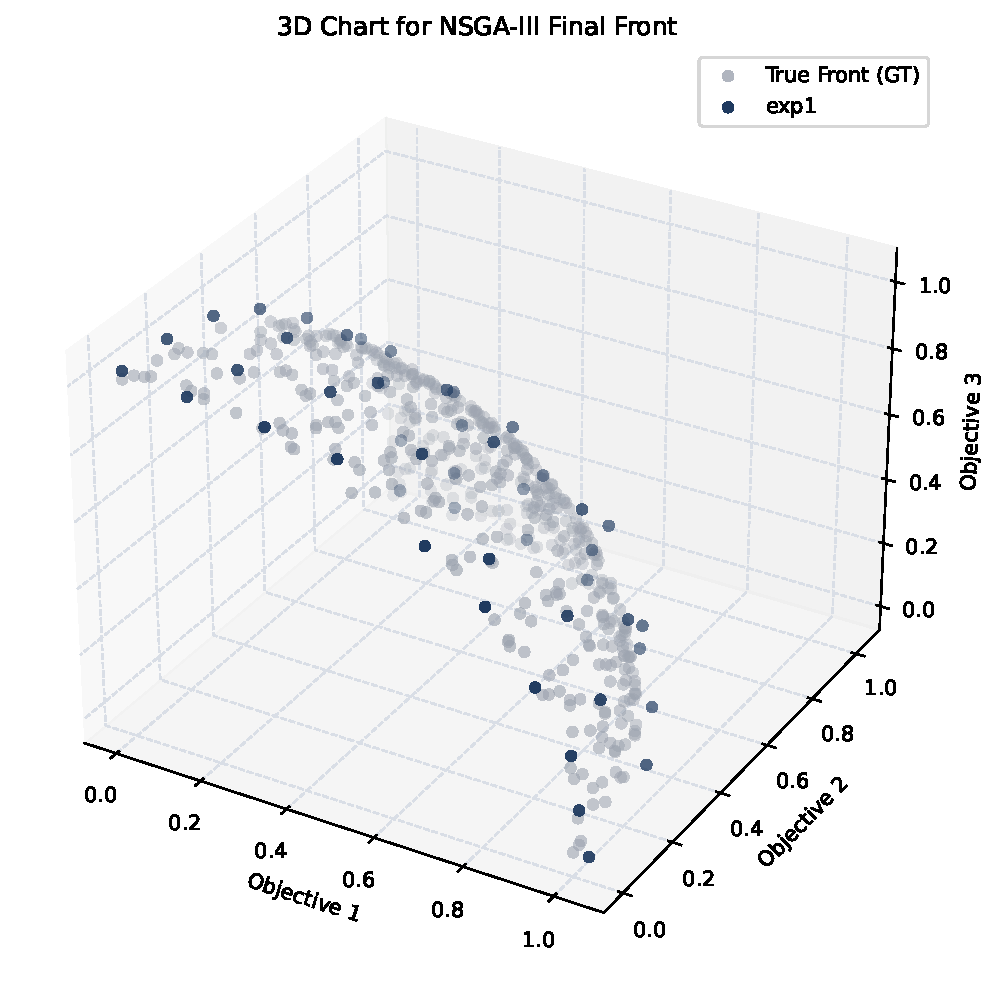
\includegraphics[width=\linewidth,height=.60\textheight,keepaspectratio]{figures/example_01_01_topology.pdf}
{\scriptsize DTLZ2 com 3 objetivos: aproximação obtida (azul) e amostragem da frente de referência (cinza).}
\end{column}
\end{columns}
\end{frame}

\begin{frame}{Experimento mínimo: evolução do desempenho}
\begin{columns}[T,onlytextwidth]
\begin{column}{.66\textwidth}
\centering
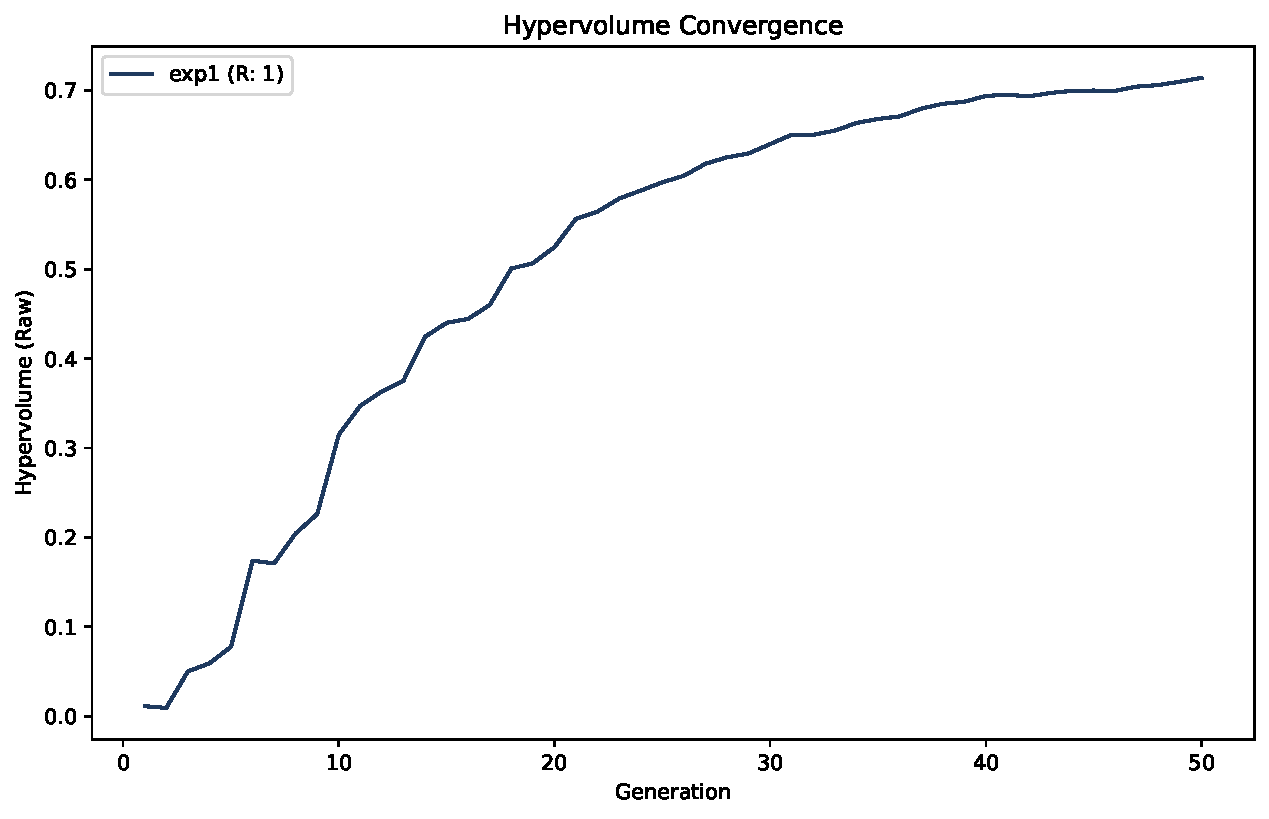
\includegraphics[width=\linewidth,height=.66\textheight,keepaspectratio]{figures/example_01_02_history.pdf}
\end{column}
\begin{column}{.32\textwidth}
\texttt{mb.view.history(exp)} apresenta, por padrão, o histórico de hypervolume.
\par\medskip
\textbf{No exemplo:} o HV aumenta durante as 50 gerações e se aproxima de um patamar ao final. A curva caracteriza o progresso da execução, enquanto a topologia mostra onde ficaram as soluções finais.
\end{column}
\end{columns}
\vspace{.15cm}{\scriptsize Figura vetorial original do exemplo 1 da monografia.}
\end{frame}

\begin{frame}[fragile]{Objetos ricos, metadados e dois espaços de análise}
\begin{columns}[T,onlytextwidth]
\begin{column}{.48\textwidth}
\centering\vspace{.2cm}
\begin{tikzpicture}[node distance=.42cm,rounded corners=1.5pt]
\node[draw=navy,thick,fill=pale,minimum width=4.2cm,minimum height=.65cm] (e) {\texttt{Experiment}};
\node[draw=black!45,fill=white,below=of e,minimum width=4.2cm,minimum height=.6cm] (r) {\texttt{Run} (cada execução)};
\node[draw=black!45,fill=white,below=of r,minimum width=4.2cm,minimum height=.6cm] (p) {\texttt{Population} (por geração)};
\node[draw=black!45,fill=white,below left=.48cm and -.65cm of p,minimum width=2cm,minimum height=.55cm] (y) {objetivos $Y$};
\node[draw=black!45,fill=white,below right=.48cm and -.65cm of p,minimum width=2cm,minimum height=.55cm] (x) {decisões $X$};
\draw[->] (e)--(r);\draw[->] (r)--(p);\draw[->] (p)--(x);\draw[->] (p)--(y);
\end{tikzpicture}
\end{column}
\begin{column}{.50\textwidth}
\begin{lstlisting}[style=python,basicstyle=\ttfamily\fontsize{8}{10}\selectfont]
exp.report()  # protocolo e metadados

# Solucoes nao dominadas:
Y = exp.front() # objetivos
X = exp.set()   # decisoes

mb.view.topology(Y)
mb.view.topology(X)
\end{lstlisting}
\vspace{.06cm}
O objeto preserva parâmetros, configurações, sementes e proveniência. As mesmas soluções podem ser examinadas no espaço de objetivos ou no espaço de decisão.
\end{column}
\end{columns}
\end{frame}

\begin{frame}[fragile]{Execuções repetidas e análise da variabilidade}
\begin{columns}[T,onlytextwidth]
\begin{column}{.60\textwidth}
\centering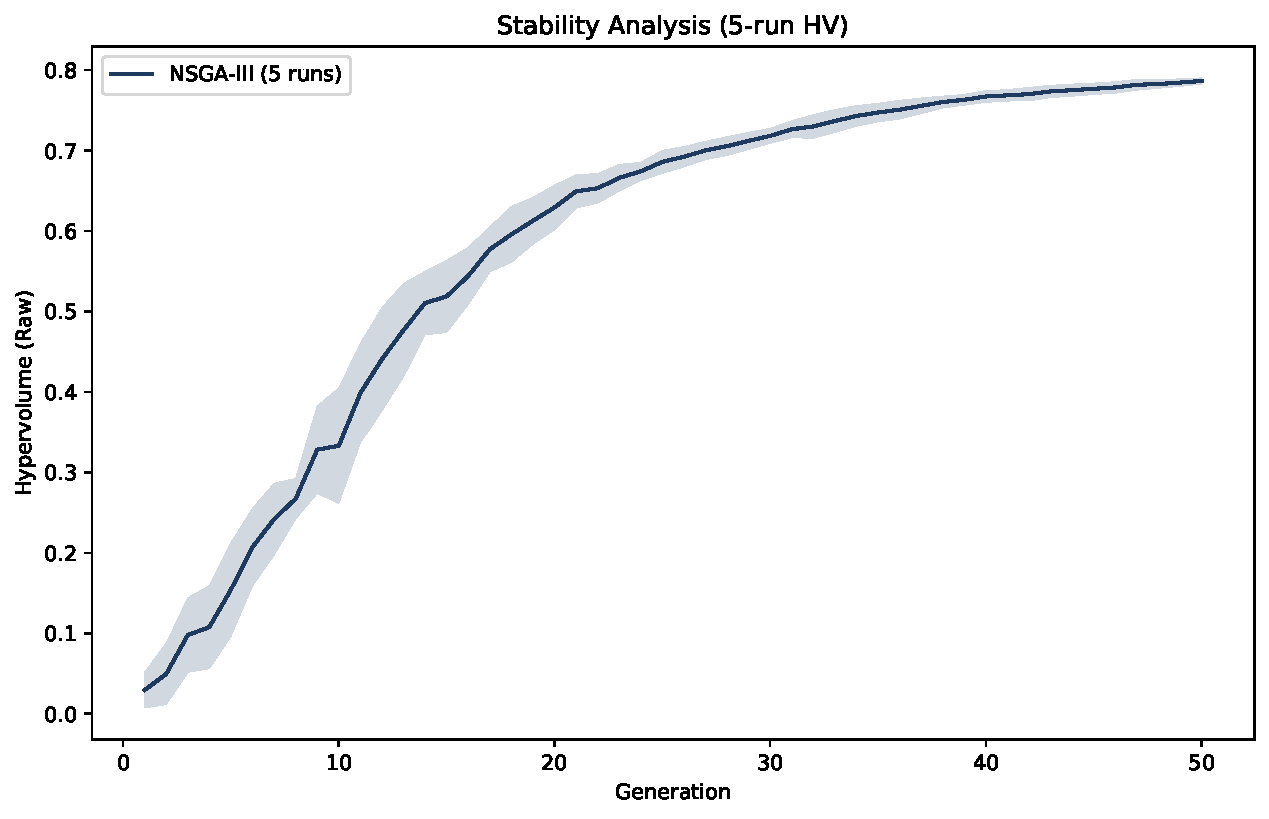
\includegraphics[width=\linewidth,height=.59\textheight,keepaspectratio]{figures/example_04_01_history.pdf}
{\scriptsize Histórico de HV de cinco execuções, com faixa de dispersão entre trajetórias.}
\end{column}
\begin{column}{.38\textwidth}
\begin{lstlisting}[style=python,basicstyle=\ttfamily\fontsize{8}{10}\selectfont]
exp.run(repeat=5)
mb.view.history(exp)
mb.view.history(exp[0])
\end{lstlisting}
\textbf{O que se vê:} as execuções apresentam maior dispersão no início; depois, as trajetórias aproximam-se e a faixa torna-se estreita. A leitura agregada não impede o exame de uma rodada individual.
\end{column}
\end{columns}
\end{frame}

\begin{frame}[fragile]{Sementes e fluxos pseudoaleatórios independentes}
\begin{columns}[T,onlytextwidth]
\begin{column}{.52\textwidth}
\begin{lstlisting}[style=python,basicstyle=\ttfamily\fontsize{8}{10}\selectfont]
exp.moea = mb.moeas.NSGA3(
    seed=42, ref_dirs_seed=7)
exp.run(repeat=3)

exp.seed     # [42, 43, 44]
exp[0].seed # 42
exp[0].component_seeds
# {'nsga3.reference_directions': 7}
\end{lstlisting}
\end{column}
\begin{column}{.46\textwidth}
A semente-base define uma sequência reproduzível de sementes para as execuções, e cada \texttt{Run} registra a semente efetivamente usada.
\par\medskip
No NSGA-III, a geração das direções de referência possui um fluxo pseudoaleatório separado daquele que conduz a evolução. O parâmetro \texttt{ref\_dirs\_seed} permite fixá-lo independentemente.
\end{column}
\end{columns}
\vspace{.1cm}
Assim, o uso de aleatoriedade por um componente auxiliar não consome inadvertidamente a sequência do processo evolutivo. Os valores integram os metadados experimentais.
\end{frame}

\begin{frame}[fragile]{Compatibilidade do ambiente e estabilidade numérica}
\begin{columns}[T,onlytextwidth]
\begin{column}{.46\textwidth}
\begin{lstlisting}[style=python,basicstyle=\ttfamily\fontsize{8}{10}\selectfont]
versions = mb.system.verify_version()
stability = mb.system.verify_stability()
comparison = mb.system.verify_experiment(exp)
\end{lstlisting}
\end{column}
\begin{column}{.52\textwidth}
\textbf{Versões:} compara dependências instaladas a um conjunto previamente validado.
\par\medskip
\textbf{Estabilidade:} executa testes numéricos explícitos, incluindo geradores pseudoaleatórios e procedimentos numéricos, comparando resultados com baselines.
\par\medskip
\textbf{Proveniência:} compara o ambiente atual com o que foi registrado no experimento.
\end{column}
\end{columns}
\vspace{.18cm}
\textbf{Exemplo de interpretação:} versões compatíveis não significam que todos os resultados serão idênticos entre ambientes; por isso, o teste numérico é distinto da conferência de versões. O relatório pode indicar estabilidade ainda não verificada.
\end{frame}

\begin{frame}[fragile]{Critérios de parada e escalabilidade}
\begin{columns}[T,onlytextwidth]
\begin{column}{.51\textwidth}
\textbf{Critérios de parada.} A política experimental pode considerar não só o número de gerações, mas também condições baseadas em qualidade, estagnação ou orçamento, por meio de uma função que recebe o estado da busca.
\begin{lstlisting}[style=python,basicstyle=\ttfamily\fontsize{8}{10}\selectfont]
exp.stop = my_stop_criterion
exp.run()
\end{lstlisting}
\end{column}
\begin{column}{.47\textwidth}
\textbf{Muitos objetivos.} O framework não impõe limites artificiais ao número de objetivos ou variáveis. Utiliza operações vetorizadas, índices espaciais para consultas de distância e aproximação por Monte Carlo quando o HV exato se torna oneroso.
\par\medskip
O relatório da métrica identifica se o cálculo foi exato ou aproximado e, neste último caso, registra amostras e semente.
\end{column}
\end{columns}
\end{frame}

\begin{frame}{Hypervolume: normalização antes da comparação}
O hypervolume mede o volume dominado relativamente a um ponto de referência. Seu valor também depende dos limites utilizados para normalizar os objetivos.
\par\medskip
\textbf{No MoeaBench:} os limites ideal e nadir são fixados a partir das frentes finais escolhidas como \texttt{ref}; os objetivos passam a uma escala normalizada e o ponto do HV é fixado em $(1{,}1,\ldots,1{,}1)$.
\[
z_i=\frac{f_i-a_i}{b_i-a_i},\qquad a_i=\min_{r\in R}r_i,\quad b_i=\max_{r\in R}r_i.
\]
\textbf{Por exemplo:} para comparar experimentos $A$ e $B$, podemos usar o mesmo $R=[A,B]$. Os dois históricos serão calculados na mesma geometria, com limites fixos durante todas as gerações.
\end{frame}

\begin{frame}[fragile]{Hypervolume: três escalas de apresentação}
\begin{columns}[T,onlytextwidth]
\begin{column}{.52\textwidth}
\begin{tabularx}{\linewidth}{@{}>{\bfseries}p{.65cm}X@{}}
raw & Volume dominado na geometria normalizada. Não há divisão por outro HV.\\[5pt]
rel & Razão entre HV calculado e o maior HV final \emph{individual} da referência adotada. \texttt{rel=1} não implica ótimo teórico.\\[5pt]
abs & Razão entre HV calculado e o HV de uma frente de referência (GT) calibrada.\\
\end{tabularx}
\end{column}
\begin{column}{.46\textwidth}
\begin{lstlisting}[style=python,basicstyle=\ttfamily\fontsize{8}{10}\selectfont]
R = [expA, expB]

mb.metrics.hv(expA, ref=R,
              scale='raw')
mb.metrics.hv(expA, ref=R,
              scale='rel')
mb.metrics.hv(expA, ref=R,
              scale='abs')
\end{lstlisting}
\end{column}
\end{columns}
\vspace{.19cm}
\textbf{Exemplo numérico hipotético, na mesma geometria:} se $HV=0{,}60$, o maior HV final de referência é $0{,}75$ e $HV_{GT}=0{,}80$, então $raw=0{,}60$, $rel=0{,}80$ e $abs=0{,}75$.
\par\smallskip{\scriptsize Na ausência de calibração compatível, a API avisa e retorna a escala raw para solicitação abs.}
\end{frame}

\begin{frame}{Três domínios de análise: espaço, desempenho e dominância}
\begin{columns}[T,onlytextwidth]
\begin{column}{.32\textwidth}
\centering
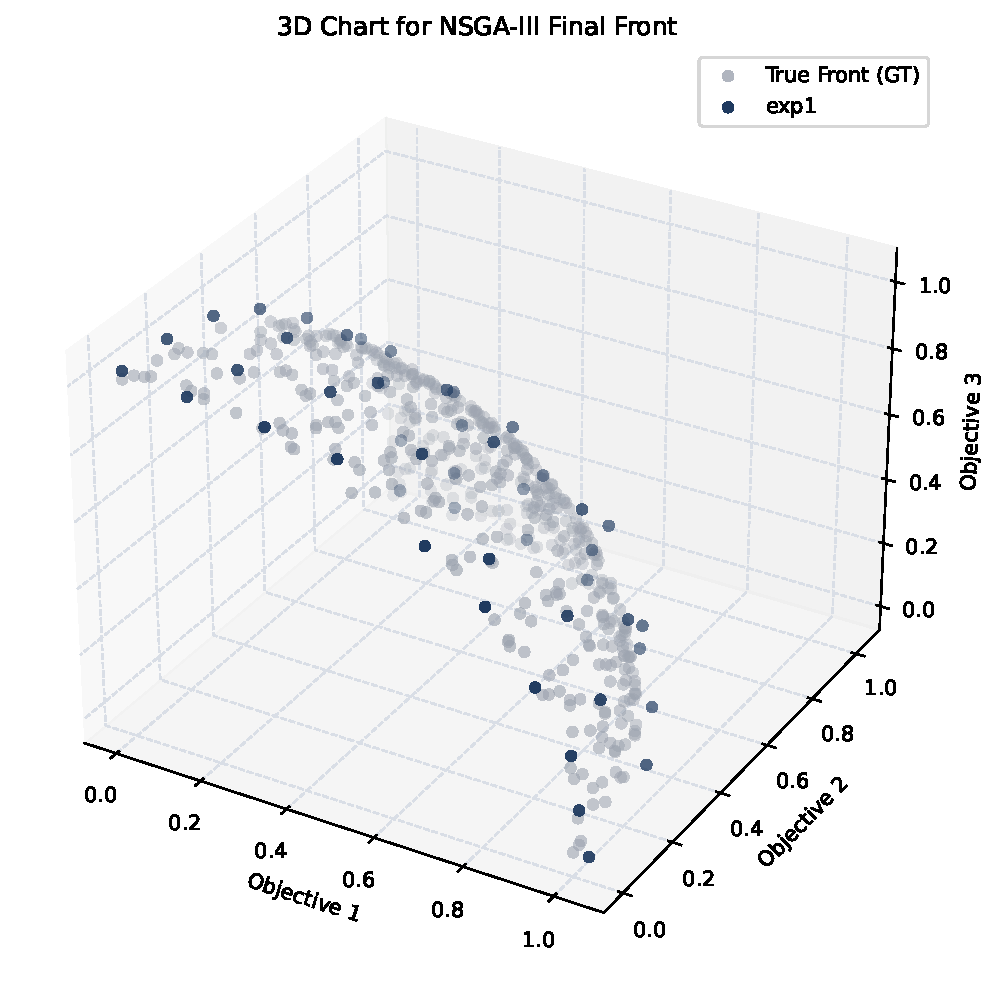
\includegraphics[width=\linewidth,height=.39\textheight,keepaspectratio]{figures/example_01_01_topology.pdf}
\par\smallskip\textbf{Topologia}\par
{\scriptsize Onde se situam as soluções no espaço dos objetivos?}
\end{column}
\begin{column}{.34\textwidth}
\centering
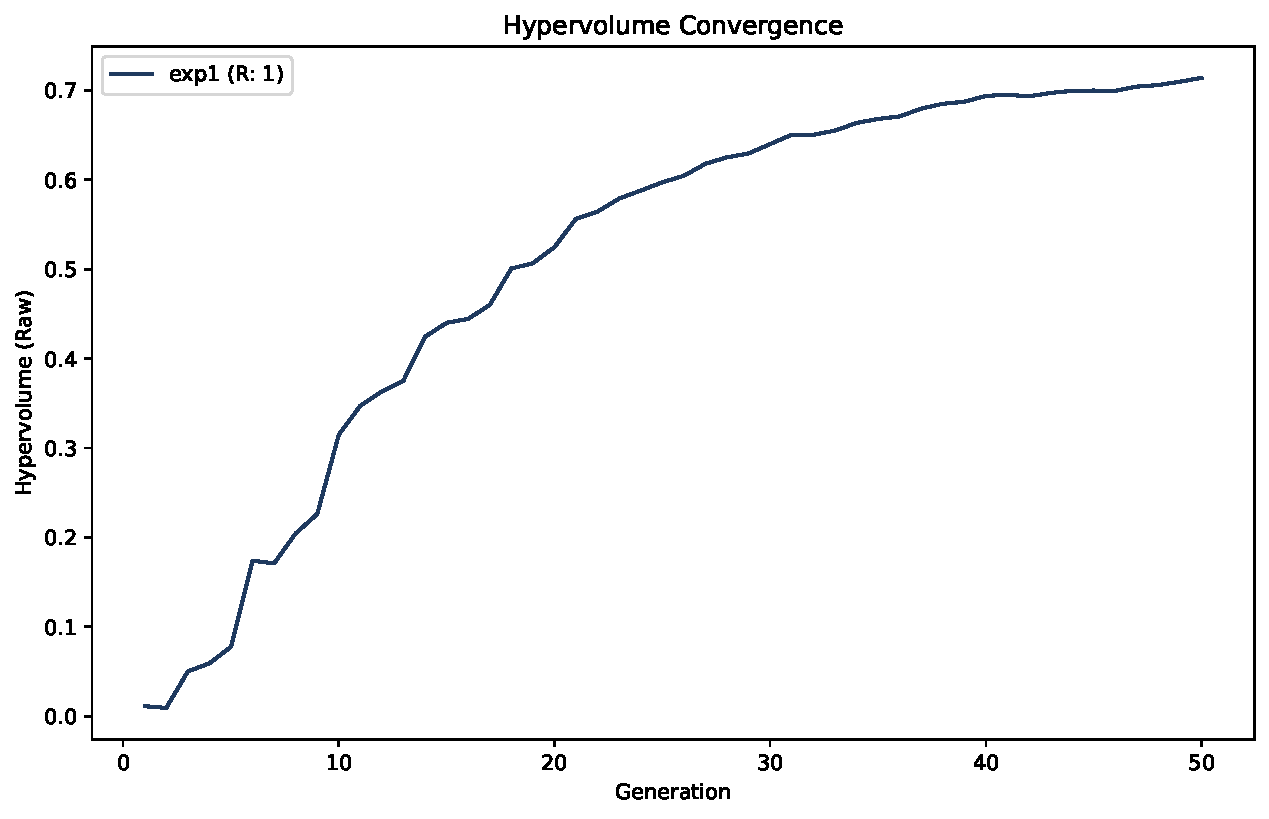
\includegraphics[width=\linewidth,height=.39\textheight,keepaspectratio]{figures/example_01_02_history.pdf}
\par\smallskip\textbf{Desempenho}\par
{\scriptsize Como o indicador evolui ao longo das gerações?}
\end{column}
\begin{column}{.32\textwidth}
\centering
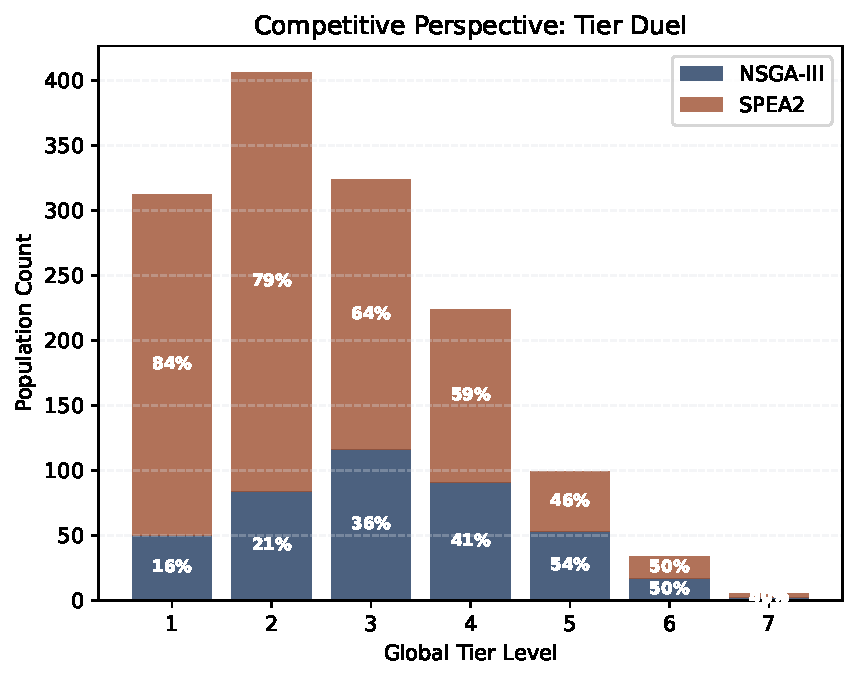
\includegraphics[width=\linewidth,height=.39\textheight,keepaspectratio]{figures/example_08_03_tiers.pdf}
\par\smallskip\textbf{Estratificação}\par
{\scriptsize Como as populações se distribuem entre ranks globais de dominância?}
\end{column}
\end{columns}
\vspace{.17cm}
Estas figuras são saídas reais dos exemplos da monografia; os três domínios respondem a perguntas complementares sobre o mesmo tipo de experimento.
\end{frame}

\begin{frame}[fragile]{Seletores: experimento, execução, filtro e espaço}
A seleção de resultados pode ser descrita por quatro decisões sucessivas, explicitadas no capítulo 4 da monografia.
\begin{center}
\begin{tikzpicture}[node distance=.10cm,>=stealth]
\node[draw=navy,fill=pale,minimum width=2.5cm,minimum height=.6cm] (a) {experimento};
\node[draw=navy,fill=pale,right=.27cm of a,minimum width=2.25cm,minimum height=.6cm] (b) {execução};
\node[draw=navy,fill=pale,right=.27cm of b,minimum width=2.05cm,minimum height=.6cm] (c) {filtro};
\node[draw=navy,fill=pale,right=.27cm of c,minimum width=2.1cm,minimum height=.6cm] (d) {espaço};
\draw[->] (a)--(b);\draw[->] (b)--(c);\draw[->] (c)--(d);
\end{tikzpicture}
\end{center}
\begin{lstlisting}[style=python,basicstyle=\ttfamily\fontsize{8}{10}\selectfont]
Y = exp[0].pop(9).objs
X = exp[0].non_dominated(9).vars
Z = exp[0].dominated(9).objs
\end{lstlisting}
Aqui, \texttt{exp[0]} escolhe a primeira execução; \texttt{pop(9)} seleciona a população completa na décima geração registrada; \texttt{.objs} devolve a matriz de objetivos. \texttt{non\_dominated()} e \texttt{dominated()} escolhem subconjuntos sem perder a correspondência entre objetivos e decisões.
\end{frame}

\begin{frame}{Seletores: atalhos ergonômicos para soluções}
\begin{tabularx}{\linewidth}{@{}>{\ttfamily}p{.31\linewidth}>{\ttfamily}p{.38\linewidth}X@{}}
\textnormal{Atalho} & \textnormal{Equivalência} & \textnormal{Significado}\\\hline
exp.front() & exp.non\_dominated().objs & Objetivos não dominados\\[8pt]
exp.set() & exp.non\_dominated().vars & Decisões não dominadas\\[8pt]
exp.non\_front() & exp.dominated().objs & Objetivos dominados\\[8pt]
exp.non\_set() & exp.dominated().vars & Decisões dominadas\\[8pt]
exp.objectives & exp.pop().objs & Objetivos de toda a população\\[8pt]
exp.variables & exp.pop().vars & Variáveis de toda a população\\
\end{tabularx}
\vspace{.26cm}
Os filtros preservam a correspondência entre soluções e valores de decisão. Os atalhos \texttt{front()} e \texttt{set()} retornam diretamente a matriz do espaço selecionado.
\end{frame}

\begin{frame}{Seletores: atalhos para execuções e referência}
\begin{tabularx}{\linewidth}{@{}>{\ttfamily}p{.33\linewidth}>{\ttfamily}p{.36\linewidth}X@{}}
\textnormal{Atalho} & \textnormal{Equivalência} & \textnormal{Significado}\\\hline
exp[0].front() & exp[0].non\_dominated().objs & Primeira execução\\[9pt]
exp[0].set() & exp[0].non\_dominated().vars & Decisões da primeira execução\\[9pt]
exp.last\_run & exp[-1] & Última execução\\[9pt]
exp.last\_pop & exp[-1].pop() & População final da última execução\\[9pt]
exp.optimal\_front() & exp.optimal().objs & Amostra da frente ótima\\[9pt]
exp.optimal\_set() & exp.optimal().vars & Amostra do conjunto ótimo\\
\end{tabularx}
\vspace{.26cm}
\texttt{optimal\_front()} e \texttt{optimal\_set()} dependem de o MOP disponibilizar uma referência; não são filtros sobre as soluções produzidas pelo algoritmo.
\end{frame}

\begin{frame}[fragile]{Seletores: resultados locais, globais e referência ótima}
\begin{columns}[T,onlytextwidth]
\begin{column}{.49\textwidth}
\begin{lstlisting}[style=python,basicstyle=\ttfamily\fontsize{8}{10}\selectfont]
# Somente a primeira execucao:
local = exp[0].front()

# Nao dominadas no conjunto
# de todas as execucoes:
global_front = exp.front()

# Amostra de referencia do MOP:
gt = exp.optimal_front()
\end{lstlisting}
\end{column}
\begin{column}{.49\textwidth}
A frente global considera a dominância entre resultados de execuções diferentes. Uma solução não dominada localmente pode ser dominada por outra rodada e desaparecer da frente global.
\par\medskip
\texttt{optimal\_front()} recupera, quando disponível, uma amostra do GT do problema; não filtra as soluções obtidas pelo MOEA.
\end{column}
\end{columns}
\end{frame}

\begin{frame}[fragile]{Delegação de seletores e resultados analíticos reutilizáveis}
\begin{columns}[T,onlytextwidth]
\begin{column}{.50\textwidth}
\textbf{Uso direto}
\begin{lstlisting}[style=python,basicstyle=\ttfamily\fontsize{8}{10}\selectfont]
mb.view.history(exp)
\end{lstlisting}
\textbf{Cálculo explícito e reuso}
\begin{lstlisting}[style=python,basicstyle=\ttfamily\fontsize{8}{10}\selectfont]
hv = mb.metrics.hv(exp)
hv.report()
mb.view.history(hv)
\end{lstlisting}
\end{column}
\begin{column}{.48\textwidth}
A visualização aceita diretamente um experimento ou um resultado previamente calculado. A API realiza a seleção necessária sem exigir que o pesquisador extraia manualmente populações e matrizes.
\par\medskip
Quando a medida será inspecionada, relatada ou reutilizada, o cálculo explícito mantém disponível o objeto analítico e seu histórico.
\end{column}
\end{columns}
\end{frame}

\begin{frame}[fragile]{Extensibilidade, persistência e reanálise}
\begin{columns}[T,onlytextwidth]
\begin{column}{.49\textwidth}
\textbf{Extensibilidade.} O pesquisador pode registrar MOPs e MOEAs personalizados e empregar sobre eles os mesmos módulos de execução e avaliação, sem alterar o núcleo da biblioteca.
\par\medskip
\textbf{Metadados.} Autoria, licença, parâmetros e informações do ambiente acompanham os resultados armazenados.
\end{column}
\begin{column}{.49\textwidth}
\textbf{Persistência.} O estado do experimento pode ser salvo, recuperado e analisado posteriormente.
\begin{lstlisting}[style=python,basicstyle=\ttfamily\fontsize{8}{10}\selectfont]
exp.save('estudo', mode='all')

# Em outra sessao, com exp criado:
exp.load('estudo', mode='all')
mb.view.topology(exp)
\end{lstlisting}
{\scriptsize A recuperação dispensa uma nova execução do algoritmo, preservando os resultados arquivados.}
\end{column}
\end{columns}
\end{frame}